% =====================================================================
%  Estimating carbohydrate and fat oxidation from heart rate
%  (paper, English version of base-teorica.tex)
%  Model of version 0.5.0. Translated on 21/11/2026.
%  Compile: pdflatex model-fc.en.tex (two passes)
% =====================================================================
\documentclass[10pt,a4paper]{article}

\usepackage[utf8]{inputenc}
\usepackage[T1]{fontenc}
\usepackage[english]{babel}
\usepackage{lmodern}
\usepackage{microtype}
\usepackage[a4paper,margin=2.4cm]{geometry}
\usepackage{amsmath,amssymb}
\usepackage{booktabs}
\usepackage{tabularx}
\usepackage{array}
\usepackage{caption}
\usepackage{pgfplots}
\pgfplotsset{compat=1.17}
\usepgfplotslibrary{groupplots}
\usepackage[numbers,sort&compress]{natbib}
\usepackage[hidelinks]{hyperref}

\captionsetup{font=small,labelfont=bf}
\renewcommand{\arraystretch}{1.25}
\newcolumntype{L}{>{\raggedright\arraybackslash}X}

\newcommand{\VO}{\ensuremath{\dot V\mathrm{O_2}}}
\newcommand{\VCO}{\ensuremath{\dot V\mathrm{CO_2}}}
\newcommand{\VOmax}{\ensuremath{\dot V\mathrm{O_{2max}}}}
\newcommand{\RER}{\ensuremath{\mathrm{RER}}}
\newcommand{\FC}{\ensuremath{\mathrm{HR}}}
\newcommand{\mlkgmin}{ml\,kg$^{-1}$\,min$^{-1}$}

\title{\textbf{Estimating carbohydrate and fat oxidation\\
from heart rate}}
\author{CHO/FAT Metabolic Pro project\\
\small\url{https://irazuzta.github.io/ChoFatMetabolic/}}
\date{Model of version 0.5.0 --- November 2026}

\begin{document}
\maketitle

\begin{abstract}
\noindent
We present a model to estimate, in real time, the rate of carbohydrate (CHO) and fat (FAT)
oxidation during exercise from a single variable that can be measured non-invasively: heart
rate (\FC). Oxygen uptake (\VO) is estimated from the equivalence between heart rate reserve
and \VO\ reserve; the respiratory exchange ratio (\RER) is approximated by a piecewise
linear interpolation anchored at four \FC\ points (exit from rest, first threshold $LT_1$,
second threshold $LT_2$ and maximum \FC). Oxidation rates are obtained with the exercise
indirect calorimetry equations of Jeukendrup and Wallis, and the cumulative total is
approximated with a Riemann sum. The \RER\ anchor values (0.86, 0.91, 0.98, 1.00) and the
relationship $LT_1\approx0.89\,LT_2$ were chosen from published measurements in trained
recreational endurance athletes on a mixed diet who exercise in the fed state. We discuss
the assumptions of the model, the factors that bias the estimate in a known direction
(fasting, low-carbohydrate diets, training status, sex, duration, heat) and the expected
precision, about $\pm20\,\%$ for CHO in a typical individual.
\end{abstract}

\noindent\textbf{Keywords:} substrate oxidation; respiratory exchange ratio; heart rate;
lactate threshold; indirect calorimetry; sports nutrition.

% ---------------------------------------------------------------------
\section{Introduction and aim}
% ---------------------------------------------------------------------

Indirect calorimetry tells us which fuel mix is being oxidised from respiratory gas
exchange, but it requires a laboratory gas analyser. The aim of this work is to obtain a
useful estimate of this information during real training, using only the \FC\ recorded by
a sports watch.

We want to know, at any instant $t$ of an activity, the oxidation rate of carbohydrate and
fat,
\begin{equation}
  CHO(t),\; FAT(t) \qquad [\mathrm{g/min}],
\end{equation}
and, from these rates, the cumulative total up to duration $T$:
\begin{equation}
  CHO_{total}(T)=\int_0^T CHO(t)\,dt, \qquad
  FAT_{total}(T)=\int_0^T FAT(t)\,dt .
  \label{eq:integral}
\end{equation}

The paper is organised as follows: section~\ref{sec:conceptes} defines the physiological
variables; sections~\ref{sec:jw}--\ref{sec:complet} build the point model ($CHO(t)$,
$FAT(t)$); section~\ref{sec:integracio} deals with time integration;
section~\ref{sec:fueling} relates the result to carbohydrate intake guidelines, and
section~\ref{sec:suposits} discusses its scope and precision.

\paragraph{Scope.} The reference values of the model are chosen for \emph{trained
recreational endurance athletes} (\VOmax\ roughly 45--60~\mlkgmin) on a \emph{normal mixed
diet} who exercise \emph{in the fed state}, at a steady effort. For other profiles (elite or
fat-adapted athletes, fasted or low-carbohydrate training, untrained people) the estimate
is biased in a known direction (section~\ref{sec:suposits}).

% ---------------------------------------------------------------------
\section{Background}\label{sec:conceptes}
% ---------------------------------------------------------------------

\subsection{Oxygen uptake and CO$_2$ output}
\VO\ is the volume of oxygen taken up per unit of time, in L/min (absolute) or in
\mlkgmin\ (relative to body mass). \VCO\ is, likewise, the volume of CO$_2$ produced.
Since oxidising fat or carbohydrate uses O$_2$ and produces CO$_2$ in different
proportions, measuring \VO\ and \VCO\ lets us infer which fuel is being burned.

\subsection{Maximal oxygen uptake}
\VOmax\ is the highest value of \VO\ a person can reach in a maximal effort, the reference
measure of cardiorespiratory capacity \citep{bassett2000}. In this model it is the upper end
of the \VO\ scale.

\subsection{Respiratory exchange ratio}
\begin{equation}
  \RER(t)=\frac{\VCO(t)}{\VO(t)} .
\end{equation}
At rest and during submaximal exercise it typically takes values between $\sim0.7$ (almost
exclusive fat oxidation) and $\sim1.0$ (almost exclusive carbohydrate oxidation). It is the
central variable of the model.

\subsection{Relative heart rate}
Absolute \FC\ is not comparable between people. The model uses the \emph{heart rate
reserve} (\%HRR), which expresses \FC\ relative to the full range between rest and maximum
\citep{karvonen1957}:
\begin{equation}
  \%HRR=\frac{\FC-\FC_{\mathrm{rest}}}{\FC_{\mathrm{max}}-\FC_{\mathrm{rest}}} .
\end{equation}

\subsection{\VO\ reserve}
In the same way, \VO\ can be expressed relative to its own range:
\begin{equation}
  \%\dot V\mathrm{O_2}R=\frac{\VO-\dot V\mathrm{O_{2,rest}}}{\VOmax-\dot V\mathrm{O_{2,rest}}} .
\end{equation}

% ---------------------------------------------------------------------
\section{Substrate oxidation equations}\label{sec:jw}
% ---------------------------------------------------------------------

The non-protein indirect calorimetry equations of \citet{frayn1983} relate \VO\ and \VCO\
to the grams of substrate oxidised. They were derived for rest, with glucose as the CHO
substrate; during exercise glycogen predominates, and \citet{jeukendrup2005} published the
modification for exercise:
\begin{align}
  CHO(t) &= 4.210\,\VCO(t)-2.962\,\VO(t), \label{eq:jw-cho}\\
  FAT(t) &= 1.695\,\VO(t)-1.701\,\VCO(t), \label{eq:jw-fat}
\end{align}
with \VO\ and \VCO\ in L/min and the result in g/min.

\subsection{Rewriting in terms of RER}
Substituting $\VCO(t)=\RER(t)\cdot\VO(t)$:
\begin{align}
  CHO(t) &= \VO(t)\,\bigl(4.210\,\RER(t)-2.962\bigr), \label{eq:cho-rer}\\
  FAT(t) &= \VO(t)\,\bigl(1.695-1.701\,\RER(t)\bigr). \label{eq:fat-rer}
\end{align}
Two independent estimates are therefore needed: \VO$(t)$ (section~\ref{sec:vo2}) and
$\RER(t)$ (sections~\ref{sec:rer}--\ref{sec:params}).

% ---------------------------------------------------------------------
\section{Estimating \VO\ from heart rate}\label{sec:vo2}
% ---------------------------------------------------------------------

The estimate is based on the empirical equivalence $\%HRR\approx\%\dot V\mathrm{O_2}R$
\citep{swain1997} (with the \VO\ reserve, not with \%\VOmax, which is less accurate):
\begin{equation}
  \dot V\mathrm{O_{2,rel}}(t)=\dot V\mathrm{O_{2,rest}}
  +\%HRR(t)\,\bigl(\VOmax-\dot V\mathrm{O_{2,rest}}\bigr),
\end{equation}
with $\dot V\mathrm{O_{2,rest}}=3.5$~\mlkgmin\ (1~MET). The absolute value is
\begin{equation}
  \VO(t)\;[\mathrm{L/min}]=\frac{\dot V\mathrm{O_{2,rel}}(t)\cdot m\;[\mathrm{kg}]}{1000}.
\end{equation}

\paragraph{Limitations.} The equivalence is a population-average approximation. The result
depends on the quality of $\FC_{\mathrm{rest}}$, $\FC_{\mathrm{max}}$ and \VOmax, which are
often estimates too. In addition, \FC\ rises at constant load with heat, dehydration or long
efforts (cardiac drift), and the model reads this as a higher intensity
(section~\ref{sec:suposits}).

% ---------------------------------------------------------------------
\section{Estimating the RER: metabolic thresholds}\label{sec:rer}
% ---------------------------------------------------------------------

The \RER\ rises non-linearly with intensity, especially around the metabolic thresholds:
$LT_1$ (aerobic threshold) and $LT_2$ (anaerobic or lactate threshold). Threshold concepts
and the validity of each definition are reviewed in \citet{faude2009}.

How the \RER\ evolves with intensity has been measured directly. In 61 trained cyclists
exercising after an overnight fast, mean \RER\ was 0.82 at rest and rose to 0.86, 0.90 and
0.98 at 41\,\%, 63\,\% and 80\,\% of $\dot V\mathrm{O_{2peak}}$, with a between-subject
standard deviation of about 0.04 at each intensity \citep{goedecke2000}.

$LT_1$ is defined as the point where blood lactate starts to rise above the resting level,
usually around 65--73\,\% of \VOmax\ in recreational runners and cyclists. The point where
the energy contribution is 50\,\% fat and 50\,\% CHO is a different concept, the
\emph{crossover point} \citep{brooks1994}, which corresponds to $\RER\approx0.85$ according
to the non-protein respiratory quotient table \citep{peronnet1991}. In a trained
recreational athlete on a normal diet this crossover occurs at low intensity: maximal fat
oxidation (\emph{Fatmax}) appears at around 48\,\% of \VOmax\ on average
\citep{venables2005}, and at $LT_1$ the \RER\ is already about 0.90.

$LT_2$ marks the maximal lactate steady state. Published \RER\ values at this point range
from about 0.90 (in steady state at the maximal lactate steady state itself) to about 0.99
(at the second ventilatory threshold in incremental tests) \citep{peinado2016}, and fat
oxidation becomes marginal. Above $LT_2$, the \RER\ can exceed 1.00 (peaks of about 1.2 in
maximal efforts) \citep{edvardsen2014}, but this excess is CO$_2$ released by bicarbonate
buffering, not additional carbohydrate oxidation. That is why the model caps the \RER\ at
1.00.

\subsection{Interpolation model}
Since lactate and gases cannot be measured outside the laboratory, the curve is
approximated with a piecewise linear interpolation between four \FC\ points: the exit from
rest $I_{on}$, $LT_1$, $LT_2$ and $\FC_{\mathrm{max}}$:
\begin{equation}
\RER(t)=
\begin{cases}
R_{basal} & \FC\le I_{on},\\[4pt]
R_{basal}+\dfrac{\FC-I_{on}}{LT_1-I_{on}}\bigl(R_{LT_1}-R_{basal}\bigr) & I_{on}<\FC\le LT_1,\\[10pt]
R_{LT_1}+\dfrac{\FC-LT_1}{LT_2-LT_1}\bigl(R_{LT_2}-R_{LT_1}\bigr) & LT_1<\FC\le LT_2,\\[10pt]
R_{LT_2}+\dfrac{\FC-LT_2}{\FC_{\mathrm{max}}-LT_2}\bigl(R_{max}-R_{LT_2}\bigr) & LT_2<\FC\le\FC_{\mathrm{max}}.
\end{cases}
\label{eq:rer}
\end{equation}

The reference values and the evidence supporting them are listed in table~\ref{tab:rer}.

\begin{table}[htbp]
\centering
\caption{RER anchor values of the model and published evidence.}
\label{tab:rer}
\small
\begin{tabularx}{\textwidth}{@{}l c L@{}}
\toprule
Point & RER & Evidence \\
\midrule
$R_{basal}$ (up to $I_{on}$; easy effort) & 0.86 &
Fasted trained cyclists: 0.82 at rest and 0.86 at 41\,\% of
$\dot V\mathrm{O_{2peak}}$ \citep{goedecke2000}; eating raises the RER at low intensity
\citep{bergman1999,achten2003cho}. Plausible range 0.82--0.90. \\
$R_{LT_1}$ & 0.91 &
$\approx0.90$ at 63\,\% of $\dot V\mathrm{O_{2peak}}$ even when fasted
\citep{goedecke2000}; $\approx0.90$--0.93 at the first ventilatory threshold in fed
recreational cyclists, estimated from published oxidation rates
\citep{martineznoguera2020}. Plausible range 0.88--0.94. \\
$R_{LT_2}$ & 0.98 &
0.976 at 80\,\% of $\dot V\mathrm{O_{2peak}}$ \citep{goedecke2000};
$\approx0.99$ at the second ventilatory threshold, but 0.90 at the maximal lactate steady
state \citep{peinado2016}. Plausible range 0.93--1.00. \\
$R_{max}$ (at $\FC_{\mathrm{max}}$) & 1.00 &
Ceiling: $\RER>1$ in near-maximal efforts is CO$_2$ from bicarbonate
\citep{edvardsen2014}, and equations~\eqref{eq:jw-cho}--\eqref{eq:jw-fat} are only valid
for $\RER\le1$. \\
\bottomrule
\end{tabularx}
\end{table}

These values describe the typical first 30--60 minutes of a steady effort in the profile
defined in section~\ref{sec:suposits}. The resulting curve rises slowly below $LT_1$ and
faster above it, which is the shape measured in trained athletes. The flat segment below
$I_{on}$ is a simplification: the real \RER\ also keeps rising with intensity in this
segment.

\paragraph{Limitations.} The interpolation assumes that the \RER\ responds instantly to
\FC\ and does not change over the effort. In reality, fat mobilisation takes a few minutes
to switch on at the start, and the \RER\ tends to fall as the effort goes on. Prior exercise
increases fat oxidation more than an overnight fast \citep{anderssonhall2016}.

% ---------------------------------------------------------------------
\section{Estimating the parameters}\label{sec:params}
% ---------------------------------------------------------------------

The model needs four \FC\ points ($I_{on}$, $LT_1$, $LT_2$, $\FC_{\mathrm{max}}$) and
\VOmax. If the athlete has had laboratory tests, the measured values are used. If not, they
have to be estimated indirectly.

\subsection{$LT_1$ as a fraction of $LT_2$}
When $LT_1$ is unknown but (an estimate of) $LT_2$ is known, it is common to approximate
the first as a fraction of the second. Group studies that have measured \FC\ at both
thresholds give ratios of about 0.88--0.91 (table~\ref{tab:lt1}).

\begin{table}[htbp]
\centering
\caption{Relationship between \FC\ at the first and second thresholds in group studies.}
\label{tab:lt1}
\small
\begin{tabularx}{\textwidth}{@{}l L l l@{}}
\toprule
Study & Population & Method & $LT_1/LT_2$ \\
\midrule
\citet{nuuttila2025} & 165 recreational runners & blood lactate &
$\approx0.89$ \\
\citet{estevelanao2026} & 1,411 runners & ventilatory thresholds & $\approx0.91$ \\
\citet{lucia2000} & elite cyclists & ventilatory thresholds & $\approx0.88$--0.90 \\
\bottomrule
\end{tabularx}
\end{table}

\noindent In \citet{nuuttila2025}, $LT_1$ and $LT_2$ were at
$80.7\pm4.9\,\%$ and $90.6\pm2.5\,\%$ of $\FC_{\mathrm{max}}$. That is why the model uses
\begin{equation}
  LT_1\approx0.89\,LT_2 .
\end{equation}
Individual variation around this ratio is large (standard deviation of 5\,\% of
$\FC_{\mathrm{max}}$, about 9~bpm) and shows only weak relationships with fitness; fixed
anchors in \%\FC\ estimated $LT_1$ with a mean absolute error of about 5--7~bpm
\citep{nuuttila2025}. A measured $LT_1$ is always preferable.

\subsection{Exit from rest, $I_{on}$}
This point does not correspond to any discrete physiological event and cannot be measured
even with a laboratory test: it is a smoothing device so that the \RER\ transition is
gradual instead of a sharp change of slope at $LT_1$. We use
\begin{equation}
  I_{on}\approx0.70\,LT_2 ,
\end{equation}
where 0.70 is a design choice, not the result of a measurement.

% ---------------------------------------------------------------------
\section{Complete point model}\label{sec:complet}
% ---------------------------------------------------------------------

Given \FC\ at an instant $t$ and the personal parameters (body mass, $\FC_{\mathrm{rest}}$,
$\FC_{\mathrm{max}}$, $LT_2$, \VOmax\ and, optionally, a measured $LT_1$), the model computes
\begin{gather}
  \FC(t)\;\longrightarrow\;\%HRR(t)\;\longrightarrow\;\VO(t),
  \qquad \FC(t)\;\xrightarrow{\eqref{eq:rer}}\;\RER(t),\notag\\
  \bigl(\VO(t),\,\RER(t)\bigr)\;\xrightarrow{\eqref{eq:cho-rer},\,\eqref{eq:fat-rer}}\;CHO(t),\;FAT(t).
\end{gather}
It is a \emph{point} model: it always answers the same question (at what rate CHO and FAT
would be oxidised if \FC\ stayed at this value), in g/min, regardless of how often it is
evaluated.

Figure~\ref{fig:model} shows the result for a reference athlete (70~kg, \VOmax\
50~\mlkgmin, $\FC_{\mathrm{rest}}=55$, $\FC_{\mathrm{max}}=185$, $LT_2=165$~bpm, and therefore
$LT_1\approx147$ and $I_{on}\approx116$~bpm).

\begin{figure}[htbp]
\centering
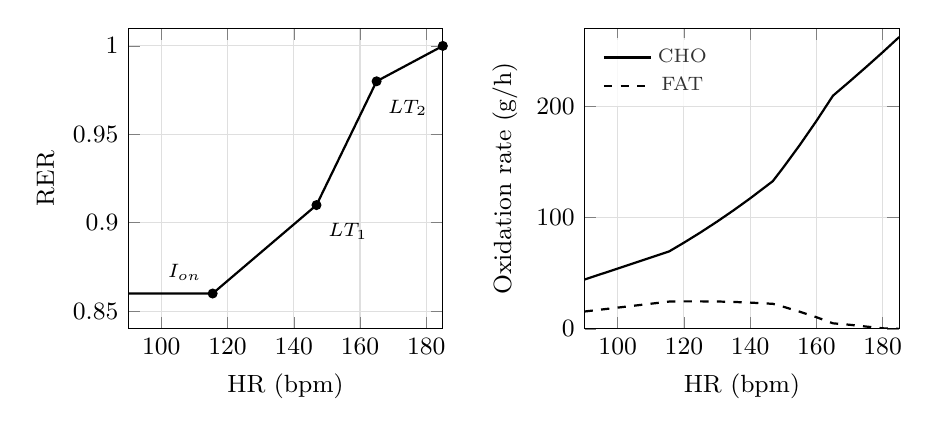
\begin{tikzpicture}
\begin{groupplot}[
  group style={group size=2 by 1, horizontal sep=1.8cm},
  width=0.46\textwidth, height=5.4cm,
  xmin=90, xmax=185, xlabel={\FC\ (bpm)},
  grid=major, grid style={gray!25},
  tick label style={font=\small}, label style={font=\small},
]
\nextgroupplot[ylabel={RER}, ymin=0.84, ymax=1.01,
  yticklabel style={/pgf/number format/fixed,/pgf/number format/precision=2}]
\addplot[thick, black] coordinates {
 (90,0.8600) (115.5,0.8600) (146.85,0.9100) (165,0.9800) (185,1.0000)};
\addplot[only marks, mark=*, mark size=1.6pt, black] coordinates {
 (115.5,0.86) (146.85,0.91) (165,0.98) (185,1.00)};
\node[font=\scriptsize, anchor=south east] at (axis cs:115,0.862) {$I_{on}$};
\node[font=\scriptsize, anchor=north west] at (axis cs:147.5,0.905) {$LT_1$};
\node[font=\scriptsize, anchor=north west] at (axis cs:165.5,0.975) {$LT_2$};
\nextgroupplot[ylabel={Oxidation rate (g/h)}, ymin=0, ymax=270,
  legend style={font=\scriptsize, at={(0.03,0.97)}, anchor=north west, draw=none, fill=white, fill opacity=0.8}]
\addplot[thick, black] coordinates {
 (90,44.3) (100,54.2) (110,64.1) (115.5,69.5) (120,77.4) (125,86.6) (130,96.3)
 (135,106.5) (140,117.2) (146.85,132.7) (150,144.9) (155,165.2) (160,186.7)
 (165,209.4) (170,222.1) (175,235.1) (180,248.4) (185,262.1)};
\addlegendentry{CHO}
\addplot[thick, dashed, black] coordinates {
 (90,15.6) (100,19.1) (110,22.6) (115.5,24.5) (120,24.7) (125,24.7) (130,24.6)
 (135,24.2) (140,23.6) (146.85,22.5) (150,19.9) (155,15.4) (160,10.5)
 (165,5.0) (170,3.7) (175,2.1) (180,0.5) (185,0.0)};
\addlegendentry{FAT}
\end{groupplot}
\end{tikzpicture}
\caption{Model for the reference athlete. Left: piecewise interpolated
\RER~\eqref{eq:rer}. Right: resulting CHO and FAT oxidation rates
\eqref{eq:cho-rer}--\eqref{eq:fat-rer}, in g/h.}
\label{fig:model}
\end{figure}

% ---------------------------------------------------------------------
\section{From instantaneous rate to cumulative total}\label{sec:integracio}
% ---------------------------------------------------------------------

\subsection{Discretisation}
Integral~\eqref{eq:integral} has no analytical solution because $\FC(t)$ is an arbitrary
function. With discrete samples $t_0=0,t_1,\dots,t_n$, the simplest approximation is the
Riemann sum:
\begin{equation}
  CHO_{total}(t_n)\approx\sum_{i=1}^{n}CHO(t_i)\,\Delta t_i, \qquad
  FAT_{total}(t_n)\approx\sum_{i=1}^{n}FAT(t_i)\,\Delta t_i,
\end{equation}
with $\Delta t_i=t_i-t_{i-1}$ in minutes. It is a first-order integration, valid when
$\Delta t$ is much smaller than the time over which the physiological state changes; if
there are large gaps, the rate of one sample is applied retroactively to the whole
interval.

\subsection{Instantaneous rate and smoothed rate}
The cumulative total answers \emph{how much I have oxidised so far}, but says nothing about
the current rate. The instantaneous rate answers \emph{how fast I am oxidising now}, but it
is noisy. A middle ground is the exponential moving average \citep{hunter1986}:
\begin{equation}
  \alpha_i\approx\frac{\Delta t_i}{\tau},\qquad
  CHO_{avg}(t_i)=CHO_{avg}(t_{i-1})+\alpha_i\bigl(CHO(t_i)-CHO_{avg}(t_{i-1})\bigr),
\end{equation}
where $\alpha_i$ is the first-order approximation of $1-e^{-\Delta t_i/\tau}$. The constant
$\tau$ is a compromise between stability and responsiveness, not a physiological property.

% ---------------------------------------------------------------------
\section{Relationship with carbohydrate intake guidelines}\label{sec:fueling}
% ---------------------------------------------------------------------

Carbohydrate intake recommendations during endurance exercise depend on duration, not on
body mass, because the limiting factor is intestinal absorption (SGLT1 and GLUT5
transporters) \citep{jeukendrup2014}:
\begin{itemize}
  \item efforts shorter than 45--60~min: no significant intake is needed;
  \item from 1 to 2--3~h: $\sim30$--60~g/h;
  \item longer than 2.5--3~h: up to $\sim90$~g/h, with multiple-transportable
        carbohydrates (glucose and fructose).
\end{itemize}
These are \emph{intake} guidelines, not oxidation targets. In moderate-to-hard exercise,
carbohydrate oxidation usually exceeds what can be absorbed, and the difference is covered
by muscle and liver glycogen. Comparing the estimated rate with these limits (about 60~g/h
with a single source, about 90~g/h with multiple transport) gives a rough idea of what part
of the effort comes from glycogen stores.

% ---------------------------------------------------------------------
\section{Assumptions, scope and precision}\label{sec:suposits}
% ---------------------------------------------------------------------

\subsection{Calibration profile}
The anchor values (table~\ref{tab:rer}) and the $LT_1/LT_2$ ratio (table~\ref{tab:lt1})
describe a typical trained recreational endurance athlete (running or cycling, \VOmax\
45--60~\mlkgmin) on a normal mixed diet (about 50--55\,\% of energy from carbohydrate), who
exercises in the fed state and without carbohydrate loading, at a steady effort and moderate
temperature, and roughly within the first hour of the effort.

\subsection{Factors that bias the estimate}
Table~\ref{tab:factors} summarises the known factors and the direction of the bias they
introduce.

\begin{table}[htbp]
\centering
\caption{Factors that move the real RER away from the model and effect on the estimate.}
\label{tab:factors}
\small
\begin{tabularx}{\textwidth}{@{}>{\raggedright\arraybackslash}p{3.6cm} L >{\raggedright\arraybackslash}p{3.4cm}@{}}
\toprule
Factor & Effect on the real RER & Effect on the estimate \\
\midrule
Fasting, low-CHO, ketogenic diet or fat adaptation &
Lower \citep{bergman1999,achten2003cho} & CHO overestimated, FAT underestimated \\
CHO-rich meal shortly before & Higher & CHO slightly underestimated \\
CHO taken during the effort & Higher & CHO slightly underestimated \\
Elite athletes & Lower at the same relative intensity ($\approx0.88$
vs.\ 0.95 at $\sim89\,\%$ of \VOmax) \citep{hetlelid2015} & CHO overestimated \\
Untrained people & Higher; \FC--\VO\ relationship and thresholds less reliable &
CHO underestimated, with more error \\
Women & Lower on average ($\approx0.03$)
\citep{rothschild2022,venables2005} & CHO slightly overestimated \\
Exercise duration & Falls by about 0.0004--0.0006 per minute \citep{rothschild2022} &
CHO increasingly overestimated from the second hour on \\
Heat, dehydration, cardiac drift & \FC\ rises at constant load; the real RER tends to
fall & \VO\ and CHO overestimated \\
Running vs.\ cycling & Higher fat oxidation when running \citep{achten2003run}; most
data are from cycling & CHO slightly overestimated when running \\
\bottomrule
\end{tabularx}
\end{table}

\subsection{Intensity range}
Equations~\eqref{eq:jw-cho}--\eqref{eq:jw-fat} were derived for moderate exercise (roughly
50--75\,\% of \VOmax) with $\RER<1$; outside this range they are an extrapolation. Above
$LT_2$ the model only counts the \emph{oxidative} use of carbohydrate: anaerobic glycolysis
also uses glycogen but does not appear in the oxidation computed from gases, so total
glycogen use in hard intervals is underestimated.

\subsection{Precision}
The individual spread of the \RER\ at a given relative intensity (standard deviation
$\approx0.04$) \citep{goedecke2000} translates, for the reference athlete at 140~bpm
($\VO\approx2.37$~L/min, $CHO\approx117$~g/h), into about $\pm24$~g/h of CHO, that is,
roughly $\pm20\,\%$:
\begin{equation}
  \Delta CHO\approx4.210\cdot\VO\cdot\Delta\RER\cdot60
  =4.210\cdot2.37\cdot0.04\cdot60\approx24~\mathrm{g/h}.
\end{equation}
To this we must add the error of the \VO\ estimate, which depends on the quality of the
inputs. The result should be read as an indication of the order of magnitude and of the
trends within a session, not as a measurement.

% ---------------------------------------------------------------------
\section{Conclusions}
% ---------------------------------------------------------------------

By combining the equivalence between \FC\ reserve and \VO\ reserve, a piecewise \RER\
interpolation anchored at the metabolic thresholds and the exercise indirect calorimetry
equations, it is possible to estimate carbohydrate and fat oxidation in real time from \FC\
alone. The chosen anchors reproduce the \RER\ values measured in fed, trained recreational
endurance athletes, and the factors that move away from them produce biases in a known
direction. With an individual precision of about $\pm20\,\%$, the model is useful to guide
carbohydrate replacement and to follow trends within a session, but it does not replace a
laboratory measurement.

% ---------------------------------------------------------------------
\begin{thebibliography}{99}
\small

\bibitem[Achten and Jeukendrup(2003)]{achten2003cho}
Achten J, Jeukendrup AE.
\newblock \emph{J Sports Sci}. 2003;21(12):1017--1024.

\bibitem[Achten et~al.(2003)]{achten2003run}
Achten J, Venables MC, Jeukendrup AE.
\newblock \emph{Metabolism}. 2003;52(6):747--752.

\bibitem[Andersson Hall et~al.(2016)]{anderssonhall2016}
Andersson Hall U, Edin F, Pedersen A, Madsen K.
\newblock Whole-body fat oxidation increases more by prior exercise than overnight
  fasting in elite endurance athletes.
\newblock \emph{Appl Physiol Nutr Metab}. 2016;41(4):430--437.

\bibitem[Bassett and Howley(2000)]{bassett2000}
Bassett DR Jr, Howley ET.
\newblock Limiting factors for maximum oxygen uptake and determinants of endurance
  performance.
\newblock \emph{Med Sci Sports Exerc}. 2000;32(1):70--84.

\bibitem[Bergman and Brooks(1999)]{bergman1999}
Bergman BC, Brooks GA.
\newblock \emph{J Appl Physiol}. 1999;86(2):479--487.

\bibitem[Brooks and Mercier(1994)]{brooks1994}
Brooks GA, Mercier J.
\newblock Balance of carbohydrate and lipid utilization during exercise: the
  ``crossover'' concept.
\newblock \emph{J Appl Physiol}. 1994;76(6):2253--2261.

\bibitem[Edvardsen et~al.(2014)]{edvardsen2014}
Edvardsen E, Hem E, Anderssen SA.
\newblock \emph{PLoS One}. 2014;9(1):e85276.

\bibitem[Esteve-Lanao et~al.(2026)]{estevelanao2026}
Esteve-Lanao J, et~al.
\newblock \emph{Sports (Basel)}. 2026;14(1):29.

\bibitem[Faude et~al.(2009)]{faude2009}
Faude O, Kindermann W, Meyer T.
\newblock Lactate threshold concepts: how valid are they?
\newblock \emph{Sports Med}. 2009;39(6):469--490.

\bibitem[Frayn(1983)]{frayn1983}
Frayn KN.
\newblock Calculation of substrate oxidation rates in vivo from gaseous exchange.
\newblock \emph{J Appl Physiol}. 1983;55(2):628--634.

\bibitem[Goedecke et~al.(2000)]{goedecke2000}
Goedecke JH, St~Clair Gibson A, Grobler L, Collins M, Noakes TD, Lambert EV.
\newblock Determinants of the variability in respiratory exchange ratio at rest and during
  exercise in trained athletes.
\newblock \emph{Am J Physiol Endocrinol Metab}. 2000;279(6):E1325--E1334.

\bibitem[Hetlelid et~al.(2015)]{hetlelid2015}
Hetlelid KJ, et~al.
\newblock \emph{BMJ Open Sport Exerc Med}. 2015;1(1):e000047.

\bibitem[Hunter(1986)]{hunter1986}
Hunter JS.
\newblock The exponentially weighted moving average.
\newblock \emph{J Qual Technol}. 1986;18(4):203--210.

\bibitem[Jeukendrup(2014)]{jeukendrup2014}
Jeukendrup AE.
\newblock A step towards personalized sports nutrition: carbohydrate intake during
  exercise.
\newblock \emph{Sports Med}. 2014;44(Suppl 1):S25--S33.

\bibitem[Jeukendrup and Wallis(2005)]{jeukendrup2005}
Jeukendrup AE, Wallis GA.
\newblock Measurement of substrate oxidation during exercise by means of gas
  exchange measurements.
\newblock \emph{Int J Sports Med}. 2005;26(Suppl 1):S28--S37.

\bibitem[Karvonen et~al.(1957)]{karvonen1957}
Karvonen MJ, Kentala E, Mustala O.
\newblock The effects of training on heart rate; a longitudinal study.
\newblock \emph{Ann Med Exp Biol Fenn}. 1957;35(3):307--315.

\bibitem[Lucía et~al.(2000)]{lucia2000}
Lucía A, et~al.
\newblock \emph{Med Sci Sports Exerc}. 2000;32(10):1777--1782.

\bibitem[Martínez-Noguera et~al.(2020)]{martineznoguera2020}
Martínez-Noguera FJ, et~al.
\newblock \emph{Nutrients}. 2020;12(12):3911.

\bibitem[Nuuttila et~al.(2025)]{nuuttila2025}
Nuuttila OP, et~al.
\newblock \emph{Eur J Appl Physiol}. 2025;125(8):2161--2171.

\bibitem[Peinado et~al.(2016)]{peinado2016}
Peinado AB, et~al.
\newblock \emph{Biol Sport}. 2016;33(4):373--380.

\bibitem[Péronnet and Massicotte(1991)]{peronnet1991}
Péronnet F, Massicotte D.
\newblock Table of nonprotein respiratory quotient: an update.
\newblock \emph{Can J Sport Sci}. 1991;16(1):23--29.

\bibitem[Rothschild et~al.(2022)]{rothschild2022}
Rothschild JA, Kilding AE, Stewart T, Plews DJ.
\newblock Factors influencing substrate oxidation during submaximal cycling: a modelling
  analysis.
\newblock \emph{Sports Med}. 2022;52(11):2775--2795.

\bibitem[Swain and Leutholtz(1997)]{swain1997}
Swain DP, Leutholtz BC.
\newblock Heart rate reserve is equivalent to \%VO$_2$ reserve, not to
  \%VO$_2$max.
\newblock \emph{Med Sci Sports Exerc}. 1997;29(3):410--414.

\bibitem[Venables et~al.(2005)]{venables2005}
Venables MC, Achten J, Jeukendrup AE.
\newblock \emph{J Appl Physiol}. 2005;98(1):160--167.

\end{thebibliography}

\end{document}
